
\documentclass[a4paper,12pt]{report}
\usepackage{xcolor}
\usepackage{color}
\usepackage[unicode]{hyperref}
\usepackage[nottoc,numbib]{tocbibind}
\hypersetup{colorlinks=true, urlcolor=green, linkcolor=black, unicode=true}
\usepackage[utf8]{inputenc}
\usepackage[utf8]{vietnam}
\usepackage{latexsym, amsfonts, amssymb, amsmath}
\usepackage[margin=2.2cm]{geometry}
\usepackage{fancybox}
\usepackage{minted}
\usepackage{frame}
\usepackage{framed}
\usepackage{graphicx}
\begin{document}
\thispagestyle{empty}
\thisfancypage{
\setlength{\fboxsep}{0pt}
\fbox}{} 
\begin{center}
    \begin{large}
        \textcolor[rgb]{1.00,0.00,0.00}{TRƯỜNG ĐẠI HỌC BÁCH KHOA HÀ NỘI}
    \end{large} \\
    \begin{large}
        \textcolor[rgb]{1.00,0.00,0.00}{VIỆN CÔNG NGHỆ THÔNG TIN VÀ TRUYỀN THÔNG}
    \end{large} \\

    \textbf{--------------------  *  ---------------------}\\[2cm]

    
\includegraphics[width=3cm, height=4.2cm]{logo}\\[1cm]
    {\fontsize{32pt}{1}\selectfont BÀI TẬP MÔN HỌC}\\
    {\fontsize{20pt}{1}\selectfont HỆ ĐIỀU HÀNH}\\[2cm]
\end{center}

%\hspace{5cm}  Đề tài 10 : Đường đi ngắn nhất trên đồ thị
\begin{flushright}
    \parbox[t]{8cm}{
    \textbf{Nguyễn Duy Thành - }CNTT1 20102737\\}%[12pt]
    %\textbf{Vũ Văn Hiệp-}CNTT2 20101545}\\[12pt]
    %\textbf{Bạch Văn Hải-}CNTT1 20101464}\\[12pt]
\end{flushright}

\hspace{5cm} Giáo viên hướng dẫn\hspace{24pt} :
\begin{flushright} \textbf{\parbox[t]{8cm}{    
        \textcolor[rgb]{0.00,0.00,1.00}{Phạm Đăng Hải}
        }}
\end{flushright}
    \vspace{2cm}
\begin{center}
        {\fontsize{16pt}{1}\selectfont HÀ NỘI}\\
        {\fontsize{16pt}{1}\today}
\end{center}

    \newpage

    \tableofcontents
    \newpage
\chapter{Lời nói đầu}
    Trong bản báo cáo này, em sẽ trình bày về chương trình shell đơn giản
    \texttt{Tiny Shell} và một số bài tập môn hệ điều hành khác. Những bài tập
    khác không trình bày ở đây nhưng vẫn có code ở file đính kèm.\\
    Những chương trình C/C++ kèm theo được biên dịch trên hệ điều hành Linux 64
    bit nên có thể phải biên dịch lại nếu không tương thích.\\

    Dù đã rất cố gắng nhưng do khả năng còn hạn chế nên không thể không có sai sót, rất
    mong được thầy tận tình chỉ bảo. Em xin chân thành cảm ơn!\\
    \begin{center}
        Sinh viên thực hiện:
        \parbox[t]{4cm}{Nguyễn Duy Thành \\ Email: boss14420@gmail.com}
    \end{center}



\chapter{Chương trình shell đơn giản (Tiny Shell) cho POSIX}:
%================Chuong I========================================
    \section{Giới thiệu}
        \subsection{Tinyshell}
        Chương trình TinyShell là một \textit{shell} dành cho Linux và các tương
        thích POSIX, có một số tính năng cơ bản như:
        \begin{itemize}
            \item Gọi, thực hiện chương trình ngoài,
            \item Thực hiện các kịch bản (\textit{script}),
            \item Liệt kê các lệnh đã gọi (\textit{history}),
            \item Gọi lại các lệnh trong \textit{history} mà không cần phải gõ lại
                (\textit{history expansion}),
            \item Quản lý tác vụ (\textit{Job control}),
            \item Làm việc với biến môi trường (\textit{Enviroment variable}),
            \item Tính toán một số phép tính số nguyên đơn giản
            \item Tab-completion
            \item Globbing
            \item \ldots{}
        \end{itemize}

        Chương trình được viết bằng ngôn ngữ C++, theo chuẩn C++11.

        \subsection{Hướng dẫn cài đặt}

        \textbf{Yêu cầu}
        \begin{itemize}
            \item Hệ điều hành: tương thích \texttt{POSIX}, với MS-Windows có thể cài
                CygWin để hỗ trợ \texttt{POSIX},
            \item \texttt{cmake} >= 2.6: để sinh \texttt{makefile}. Download ở \\
                \href{http://www.cmake.org/cmake/resources/software.html}{\texttt{http://www.cmake.org/cmake/resources/software.html}}.\\
                Với Linux có thể cài đặt qua các \texttt{package manager}
            \item thư viện \texttt{GNU readline},             
	    \item trình dịch: tốt nhất là \texttt{gcc >= 4.6}, với các trình dịch
                khác cần phải sửa file \texttt{CMakeLists.txt}.
        \end{itemize}

        \textbf{Với các Linux distro họ Debian (Debian, Ubuntu, Mint, ...)}:
            Cài đặt một trong những gói phần mềm (file .deb) đi kèm, tuỳ loại
            kiến trúc là 32bit và 64bit.\\
            Ví dụ \texttt{Ubuntu 32bit}, nháy đúp chuột vào file
            \texttt{tinyshell\_0.1-1\_i386.deb} để vào chương trình cài đặt
            gói, hoặc dùng lệnh:
                \begin{minted}[frame=single,linenos=true,tabsize=4]{bash}
$ sudo dpkg -i tinyshell_0.1-1_i386.deb
                \end{minted}

        \textbf{Với các hệ điều hành khác}:
            Cần phải biên dịch lại từ mã nguồn. Các bước tiến hành như sau:
        \begin{enumerate}
            \item \textbf{Sinh \texttt{Makefile}}: vào thư mục gốc của mã nguồn
                \texttt{Tinyshell}, gõ lệnh:
                \begin{minted}[frame=single,linenos=true,tabsize=4]{bash}
$ cmake CMakeLists.txt
                \end{minted}
                Nếu có lỗi xảy ra thì có nghĩa là một số thư viện cần thiết
                chưa được cài đặt.
            \item \textbf{Biên dịch và cài đặt}, gõ lệnh:
                \begin{minted}[frame=single,linenos=true,tabsize=4]{bash}
$ make
$ sudo make install # can quyen root
                \end{minted}
                file thực thi \texttt{tinyshell} sẽ được tạo ra và sao chép vào
                thư mục \texttt{/usr/bin}.
        \end{enumerate}
%==========================finish Chuong I===========================

%==============Chuong II=============================================
%-------------section 2.1 -------------------------------------------
    \section{Khởi động chương trình}
    Mở chương trình, gõ lệnh:
    \begin{minted}[frame=single,linenos=true,tabsize=4]{bash}
$ tinyshell
    \end{minted}
    \begin{figure}
        \centering
        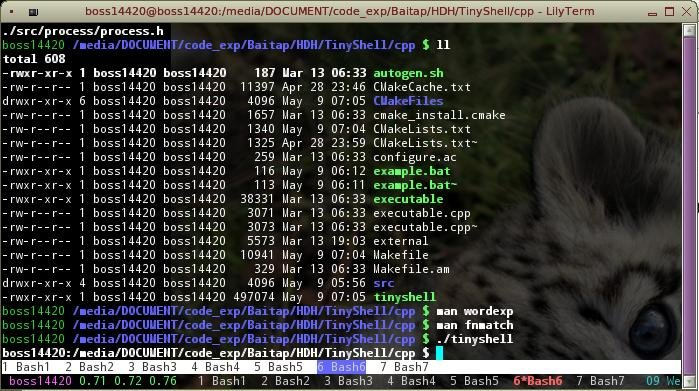
\includegraphics[scale=0.7]{ts1}
        \rule{35em}{0.5pt}
        \caption{Tiny Shell}
        \label{fig:ts1}
    \end{figure}

    Từ \texttt{bash} shell(mặc định trên Linux) sẽ chuyển sang tinyshell. Hình
    \ref{fig:ts1}. Dấu nhắc lệnh của \texttt{Tiny Shell} có dạng
    \texttt{<username>:<current working directory> \$}, nếu $username$ có $root$ thì
    kết thúc dấu nhắc lệnh là \#.

    Để kết thúc \texttt{Tiny Shell}, dùng tổ hợp phím \texttt{Ctrl+D} hoặc gõ
    lệnh \texttt{quit}.

    %-------------section 2.2 -------------------------------------------
    \section{Gọi lệnh}
    Với \texttt{Tiny Shell}, ta có thể gõ lệnh bình thường như các
    \textit{shell} khác:
    \begin{minted}[frame=single,linenos=true,tabsize=4]{bash}
$ ls -liah # thuc thi chuong trinh ngoai
$ ./abc.py # thuc thi file script python
    \end{minted}

    Chú ý:
    \begin{itemize}
        \item Nếu ghi đường dẫn (tương đối hoặc tuyệt đối) thì \texttt{Tiny
            Shell} sẽ tìm kiếm file thực thi trong các thư mục được lưu
            trong biến môi trường \texttt{PATH}. \\
            VD: với \texttt{PATH = /usr/bin/:/bin:/usr/local/bin} \\
            thì \texttt{Tiny Shell} sẽ tìm
            kiếm file thực thi trong các thư mục \texttt{/usr/bin/},
            \texttt{/bin}, \texttt{/usr/local/bin}.
        \item Nếu không tìm thấy file thực thi thì \texttt{Tiny Shell} sẽ
            báo lỗi \texttt{bad command}.
        \item Chỉ có nhưng file có \texttt{execute permission} mới có quyền
            thực thi. VD, với file có \texttt{permission/mode} là 422
            ($---x-w--w-$) thì chỉ có \texttt{owner} của file mới được thực
            thi. Những người dùng khác nếu thực thi file này sẽ bị báo lỗi
            \texttt{permission denied}.
            chỉ có \texttt{owner} của file mới được quyền thực thi.
        \item File script phải bắt đầu bằng 2 kí tự \texttt{sha-bang (\#!)},
            tiếp theo là câu lệnh (có thể có cả tham số) để thực hiện
            chương trình đó. Chẳng hạn, một python script phải có dòng đầu
            tiên là:\\
            \begin{minted}[frame=single,linenos=true,tabsize=4]{bash}
#!/usr/bin/env python
            \end{minted}
    \end{itemize}

    Để bắt buộc chương trình kết thúc, dùng tổ hợp phím \texttt{Ctrl+C}
    (một số chương trình có thể bỏ qua yêu cầu này).

    Để tạm dừng chương trình, dùng tổ hợp phím \texttt{Ctrl+Z}. Xem thêm ở mục 
    \textcolor{blue}{\ref{sec:jobcontrol}}.

%-------------section 2.3 -------------------------------------------
    \section{Lệnh nâng cao}
    \texttt{Tiny Shell} sử dụng hàm \texttt{wordexp} của \texttt{libc}
    nên có thể thực hiện được một số thay thể các từ mà người dùng nhập vào
    tương tự \texttt{bash shell}. \cite{LCWE}. Ví dụ:
    \begin{minted}[frame=single,linenos=true,tabsize=4]{bash}
$ # liet ke thu muc goc cua nguoi dung boss14420
$ ls ~boss14420
...
$ # xem bien moi truong $PATH
$ echo $PATH
...
$ # Phep tinh so hoc
$ echo $(( 2*3 ))
...
$ # tam dung tien trinh firefox
$ kill -STOP `pidof firefox`
...
$ # liet ke nhung file co phan mo rong la .c
$ ls *.c
$ # xoa nhung file co dang abc.<chu so> trong thu muc
$ rm abc.[0-9]
    \end{minted}
(Chú ý, kí tự ` tương ứng với phím ở bên trái phím số 1 trên bàn phím).

%-------------section 2.4 -------------------------------------------
    \section{Job control}
    \label{sec:jobcontrol}
    \texttt{Tiny Shell} có một số tính năng của một \texttt{Job Control}
    shell \cite{LCJC}.
        \subsection{Background/foreground}
	    Một chương trình được gọi từ \texttt{Tiny Shell} có thể thực thi
	    theo hai chế độ : chế độ hiện (\texttt{foreground}) và chế độ nền
	    \texttt{background}. Ở chế độ hiện thì chương trình được gọi sẽ
	    nhận dữ liệu từ \texttt{stdin} (thay vì \texttt{Tiny Shell}), tức
	    là người dùng chỉ có thể giao tiếp với chương trình chứ không thể
	    giao tiếp với \texttt{Tiny Shell} được nữa. Còn ở chế độ nền thì
	    người dùng có thể giao tiếp với \texttt{Tiny Shell} trong khi
	    chương trình đang chạy, chương trình không thể nhận dữ liệu từ
	    người dùng nhưng vẫn có thể xuất dữ liệu ra ngoài. Để chạy chương
	    trình ở chế độ nền thì thêm \texttt{\&} ở cuối câu lệnh. Ví dụ:
	
	    \begin{minted}[frame=single,linenos=true,tabsize=4]{bash}
$ ./external 
Sleeping...
Waked!
$ 
$ ./external &
$ Sleeping...

$ ls
autogen.sh      CMakeFiles      CMakeLists.txt  configure.ac    
example.bat~    executable.cpp  external        Makefile.am     
tinyshell       CMakeCache.txt  cmake_install.cmake 
CMakeLists.txt~ example.bat     executable      executable.cpp~  
Makefile        src
$ Waked!

[1]     Done            ./external 
$ 
	    \end{minted}
	
        \subsection{Liệt kê các tiến trình nền}
	    Dùng lệnh \texttt{jobs} để liệt kê các tiến trình nền đang chạy.
	    Nội dung kết quả gồm nhiều dòng, một dòng tương ứng một tiến trình
	    nền, có dạng:
	    \begin{minted}[frame=single,linenos=true,tabsize=4]{bash}
[<id>]<default>      <status>         <command>
	    \end{minted}
	    Trong đó:
	    \begin{itemize}
	        \item \texttt{<id>} là chỉ số của tiến trình, dùng để phân biệt
	            với các tiến trình khác,
	        \item Nếu \texttt{<default>} là '+', tiến trình sẽ là tiến
	            trình mặc định cho các lệnh \texttt{fg, bg} (sẽ nói phần
	            tiếp theo). Nếu \texttt{<default>} là '-', tiến trình sẽ
	            trở thành mặc định khi tiến trình mặc định kết thúc. Chỉ có
	            tối đa một tiến trình '+' và một tiến trình '-'.
	        \item \texttt{<status>} là trạng thái của tiến trình. Có hai
	            trạng thái là
	            \texttt{Running} có nghĩa là tiến trình đang chạy,
	            \texttt{Stopped} có nghĩa là tiến trình đã bị dừng lại do
	            người dùng gửi tín hiệu dừng \texttt{STOP signal} đến tiến
	            trình bằng tổ hợp phím \texttt{Ctrl+Z},
	        \item \texttt{<command>} là câu lệnh shell.
	    \end{itemize}
	
	    Ví dụ:
	    \begin{minted}[frame=single,linenos=true,tabsize=4]{bash}
$ vim
[1]+    Stopped         vim
$ less example.bat
[2]+    Stopped         less example.bat
$ ./external 6 &
$ Sleeping...

$ jobs
[1]-    Stopped         vim
[2]+    Stopped         less example.bat
[3]     Running         ./external 6 
$
	    \end{minted}
	
        \subsection{Chuyển từ \texttt{foreground} sang
	    \texttt{background}}
	    Đôi khi có những chương trình cần thời gian thực hiện dài (ví
	    dụ chương trình tính toán, chương trình chơi nhạc) mà cần một
	    số dữ liệu đầu vào do người dùng nhập. Rõ ràng không thể bắt
	    đầu chương trình ở chế độ \texttt{background} (vì cần nhập dữ
	    liệu) và cũng không thể đợi chương trình chạy xong mới tiếp tục
	    làm việc với \texttt{Tiny Shell}. Hay có nhiều chương trình ta
	    muốn chạy ở chế độ \texttt{background} nhưng lại quên thêm dấu
	    \texttt{\&} ở cuối câu lệnh, ta cũng không thể chờ chương trình
	    chạy xong hoặc tắt chương trình để chạy lại.\\
	
	    Với những trường hợp như trên, ta có thể chuyển tiến trình từ
	    \texttt{foreground} sang \texttt{background} lúc cần thiết, như
	    vậy chương trình vẫn chạy mà ta vẫn có thể làm việc khác.
	
	
	    Ta thực hiện như sau:\\
	
	    Vì lúc này người dùng không thể tương tác với\texttt{Tiny
	    Shell} nên trước hết phải cho tiến trình tạm dừng bằng tổ hợp
	    phím \texttt{Ctrl+Z}.\\
	    Sau đó, đưa tiến trình về chế độ \texttt{background} và tiếp
	    tục tiến trình, dùng lệnh \texttt{bg}. Cú pháp lệnh \texttt{bg}
	    như sau:
	    \begin{minted}[frame=single,linenos=true,tabsize=4]{bash}
bg [job_id ...]
	    \end{minted}
	    Trong đó, \texttt{job\_id} là danh sách chỉ số của các tiến
	    trình (đã bị tạm dừng) muốn đưa về chế độ nền. Nếu không chỉ ra
	    \texttt{job\_id} thì tiến trình được chọn sẽ là tiến trình mặc
	    định (tức tiến trình có kèm theo dấu '+' trong kết quả liệt kê
	    bằng lệnh \texttt{jobs}. Một tiến trình sẽ trở thành tiến trình
	    mặc định khi nó là tiến trình gần nhất bị tạm dừng. Ví dụ:
	    \begin{minted}[frame=single,linenos=true,tabsize=4]{bash}
$ mpg123 "abcde.mp3"
High Performance MPEG 1.0/2.0/2.5 Audio Player for Layers 1, 2 and 3
version 1.14.1; written and copyright by Michael Hipp and others
free software (LGPL/GPL) without any warranty but with best wishes

Playing MPEG stream 1 of 1: abcde.mp3 ...

MPEG 1.0 layer III, 192 kbit/s, 44100 Hz joint-stereo
Title:   dam Ma (Remix)                  Artist: DJ
Comment: NhacCuaTui.Com - Nghe Nhac Moi Luc Moi Noi
Album:   NhacCuaTui.Com
Year:    2011                            Genre:  The Loai Khac
^Z[2]+  Stopped         mpg123 "abcde.mp3"
$ bg
$ # lam cong viec khac trong khi mpg123 van tiep tuc choi nhac
	    \end{minted}
	
        \subsection{Chuyển tiến trình sang \texttt{foreground}}
	    Ngược lại với phần trên, giả sử có những chương trình đang chạy ở
	    \texttt{background} hoặc chương trình đang tạm dừng muốn chuyển về
	    \texttt{foreground}. Ta có câu lệnh \texttt{fg}
	    \begin{minted}[frame=single,linenos=true,tabsize=4]{bash}
	    fg [job_id]
	    \end{minted}
	
	    Trong đó \texttt{job\_id} là chỉ số của tiến trình muốn chuyển về
	    \texttt{foreground}. Nếu không chỉ ra \texttt{job\_id} thì chọn
	    tiến trình mặc định (tương tự lệnh \texttt{fg}). Ví dụ:
	    \begin{minted}[frame=single,linenos=true,tabsize=4]{bash}
$ # dung vim de soan thao ma nguon
$ vim source.c
[1]+    Stopped         vim source.c
$ # tam dung de bien dich va chay thu
$ gcc source.c -o source -Wall -O2
$ ./source
...
$ # tiep tuc sua file source.c
$ fg
	    \end{minted}

        \subsection{Kết thúc một tiến trình}
            \texttt{Tiny Shell} cung cấp lệnh \texttt{kill} dùng để gửi một
            \texttt{tín hiệu (signal)} đến một tiến trình. Chức năng của lệnh
            \texttt{kill} giống như lệnh \texttt{kill} của \texttt{GNU Biutils}
            nhưng có thêm tính năng gửi \texttt{signal} đến các tiến trình
            \texttt{nền} của \texttt{Tiny Shell} dựa trên \texttt{job\_id}
            (bằng cách thêm \texttt{\%} vào trước chỉ số) thay
            vì \texttt{pid}. Ví dụ:
            \begin{minted}[frame=single,linenos=true,tabsize=4]{bash}
$ ./external 10 &
$ Sleeping...

$ jobs
[1]     Running         ./external 10 
$ kill %1
[1]     Done            ./external 10 
$ 
$ # Tiep tuc tien trinh khac
$ kill -CONT `pidof firefox`
$
            \end{minted}
            Thông tin về cú pháp của lệnh \texttt{kill} xem thêm ở
            \texttt{manual} (dùng lệnh \texttt{man 1 kill}).

%-------------section 2.5 -------------------------------------------
    \section{Một số tiện ích khi gõ lệnh}
        Do \texttt{Tiny Shell} giao tiếp với người dùng chủ yếu qua lệnh nên có
        một số tính năng để công việc này nhẹ nhàng hơn:
        \subsection{Tab-completion}
        \begin{figure}
            \centering
            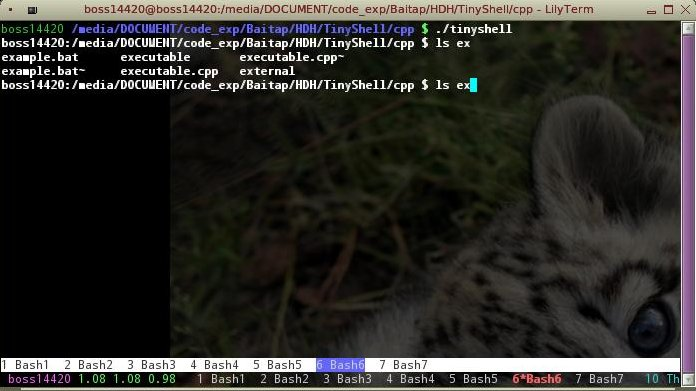
\includegraphics[scale=0.7]{ts2}
            \rule{35em}{0.5pt}
            \caption{Tab-completion}
            \label{fig:ts2}
        \end{figure}
        Khi lệnh có chứa tên một đường dẫn có thực hoặc một file có trong
        thư mục hiện tại thì ta chỉ cần gõ một số kí tự đầu và sau đó nhấn
        phím \texttt{Tab} 2 lần, \texttt{Tiny Shell} sẽ tự động hoàn thành.
        Nếu có nhiều file có tên bắt đầu trùng với các ký tự đã gõ thì
        những tên file đó sẽ được in ra (Hình \ref{fig:ts2}).

        \subsection{Lịch sử - History}
        Mỗi khi người dùng thực thi một lệnh bằng \texttt{Tiny Shell} (có thể
        lỗi) thì lệnh đó được lưu vào \texttt{history}. Người dùng sau này có
        thể gọi lại các lệnh đã gõ mà không cần phải gõ lại tất cả.
        \begin{itemize}
            \item Để hiển thị tất cả các câu lệnh đã thực thi, dùng lệnh
                \texttt{history}
                \begin{minted}[frame=single,linenos=true,tabsize=4]{bash}
$ ls
...
$ shfdjskj
$ history
1. ls
2. shfdjskj
$
                \end{minted}
            \item Dùng các phím mũi tên lên/xuống để thay câu lệnh đang gõ dỡ
                bằng các câu lệnh trước/sau.
            \item Để thực hiện câu lệnh thứ $n$ trong \texttt{history}, dùng
                lệnh \texttt{!n}
            \item Để thực hiện câu lệnh thứ $n$ \textit{tính từ câu lệnh hiện
                tại}, ta dùng lệnh \texttt{!-n}. Ví dụ, để thực hiện câu lệnh
                gần nhất, ta dùng lệnh \texttt{!-1}.
            \item Nếu không nhớ thứ tự các câu lệnh, vẫn có thể gọi lại mà chỉ
                cần gõ một vài kí tự đầu. Lệnh \texttt{!<string>} sẽ thực thi
                câu lệnh gần nhất bắt đầu bằng \texttt{<string>}. Với ví dụ
                trên, lệnh \texttt{!h} tương đương gọi lại lệnh liệt kê lịch
                sử.
            \item \ldots{}
        \end{itemize}

        \subsection{Chú thích - \texttt{comment}}
        Tất cả nhưng kí tự kể từ \texttt{\#} (không nằm trong dấu nháy đơn
        hoặc nháy kép) cho đến kết thúc dòng đều được \texttt{Tiny Shell}
        bỏ qua:
        \begin{minted}[frame=single,linenos=true,tabsize=4]{bash}
$ # Day la mot comment
$ echo " day # khong phai la mot comment "
day # khong phai la mot comment
$
        \end{minted}

%-------------section 2.6 --------------------------------------------
    \section{Các lệnh có sẵn của\texttt{Tiny Shell}} 
        Ngoài các lệnh \texttt{kill, history, fg, bg, jobs} đã đề cập,
        \texttt{Tiny Shell} còn tích hợp một số lệnh khác:
        
        \subsection{Thay đổi thư mục hiện tại - lệnh \texttt{cd}}
            Cú pháp lệnh cd như sau:
            \begin{minted}[frame=single,linenos=true,tabsize=4]{bash}
cd [new_dir]
            \end{minted}
            \texttt{new\_dir} là thư mục sẽ chuyển đến.\\
            Trong đó:
            \begin{itemize}
                \item Nếu không chỉ ra \texttt{new\_dir} thì sẽ chuyển đến thư
                    mục gốc của người dùng hiện tại,
                \item Nếu \texttt{new\_dir} là \texttt{\-} thì thư mục được
                    chuyển tới là thư mục trước đó (thư mục trước khi chuyển
                    đến thư mục hiện tại),
                \item Nếu \texttt{new\_dir} là \texttt{..} thì chuyển đến thư
                    mục cha của thư mục hiện tại
            \end{itemize}
            Ví dụ:
            \begin{minted}[frame=single,linenos=true,tabsize=4]{bash}
boss14420:/media/DATA/Music $ cd ../Video
boss14420:/media/DATA/Video $ 
boss14420:/media/DATA/Video $ # Ve thu muc goc
boss14420:/media/DATA/Video $ cd
boss14420:/home/boss14420 $
boss14420:/home/boss14420 $ # Den thu muc cha
boss14420:/home/boss14420 $ cd ..
boss14420:/home $
boss14420:/home $ # tro ve thuc muc goc
boss14420:/home $ cd -
boss14420:/home/boss14420 $
            \end{minted}

        \subsection{Xem thông tin về các lệnh khác - lệnh \texttt{help}}
            Để xem danh sách tất cả các lệnh tích hợp sẵn của \texttt{Tiny
            Shell}, dùng lệnh \texttt{help}.\\
            Để xem thông tin về một lệnh nào đó (ví dụ \texttt{cd}), dùng lệnh:
            \begin{minted}[frame=single,linenos=true,tabsize=4]{bash}
help cd
            \end{minted}

%-------------section 2.6 -------------------------------------------
	\section{Xử lí theo lô - \texttt{batch processing}}
        Thay vì gõ từng dòng lệnh, người dùng có thể xử thực thi một lúc nhiều
        lệnh khác nhau, những lệnh này được lưu vào trong một file script.\\
        File script của \texttt{Tiny Shell} có cấu trúc tương tự các shell
        script khác: các lệnh được viết trên một dòng, có thể bao gồm các
        comment, có thể chạy nền hoặc ẩn. Ví dụ, file \texttt{example.tsh}:
        \begin{minted}[frame=single,linenos=true,tabsize=4]{bash}
#!/usr/bin/tinyshell -f
# luon phai bat dau bang dong nhu tren
ls -1
# build
$ gcc abc.c -o abc
        \end{minted}
        Thực thi file này:
\begin{minted}[frame=single,linenos=true,tabsize=4]{bash}
$ # them quyen thuc thi
$ chmod +x example.tsh
$ # thuc thi nhu mot file script binh thuong
$ ./example.tsh
$
$ # hoac co the goi qua Tiny Shell, bang cach nay thi khong can file co quyen
$ # thuc thi
$ tinyshell -f example.tsh
        \end{minted}

        File script \texttt{Tiny Shell} có thể thực thi trên các shell khác.
%-------------section 2.7 -------------------------------------------
	\section{Gọi \texttt{Tiny Shell} từ các shell khác}
        Để thực thi một câu lệnh bằng \texttt{Tiny Shell} từ một shell khác,
        dùng lệnh:
        \begin{minted}[frame=single,linenos=true,tabsize=4]{bash}
$ tinyshell -c "<command>"
$ 
$ # hoặc
$ tinyshell --command="<command>"
$
        \end{minted}

        Để thực thi file script:
        \begin{minted}[frame=single,linenos=true,tabsize=4]{bash}
$ tinyshell -f "<file>"
$
$ # hoac
$ tinyshell --script="<file>"
$
        \end{minted}

        Có thể gọi \texttt{Tiny Shell} ngay từ chính \texttt{Tiny Shell}.

%========================Phan II================================

\chapter{Một số bài tập môn Hệ Điều Hành}

        \include{producer-consumer}
        \include{chat}
        \include{reader-writer}
        \include{mbr}
%======================REFERENCE================================

\bibliographystyle{plain}
\bibliography{reference}

%==================================finish=========================

\end{document}
